\begin{figure}
    \begin{fullwidth}
    \centering
    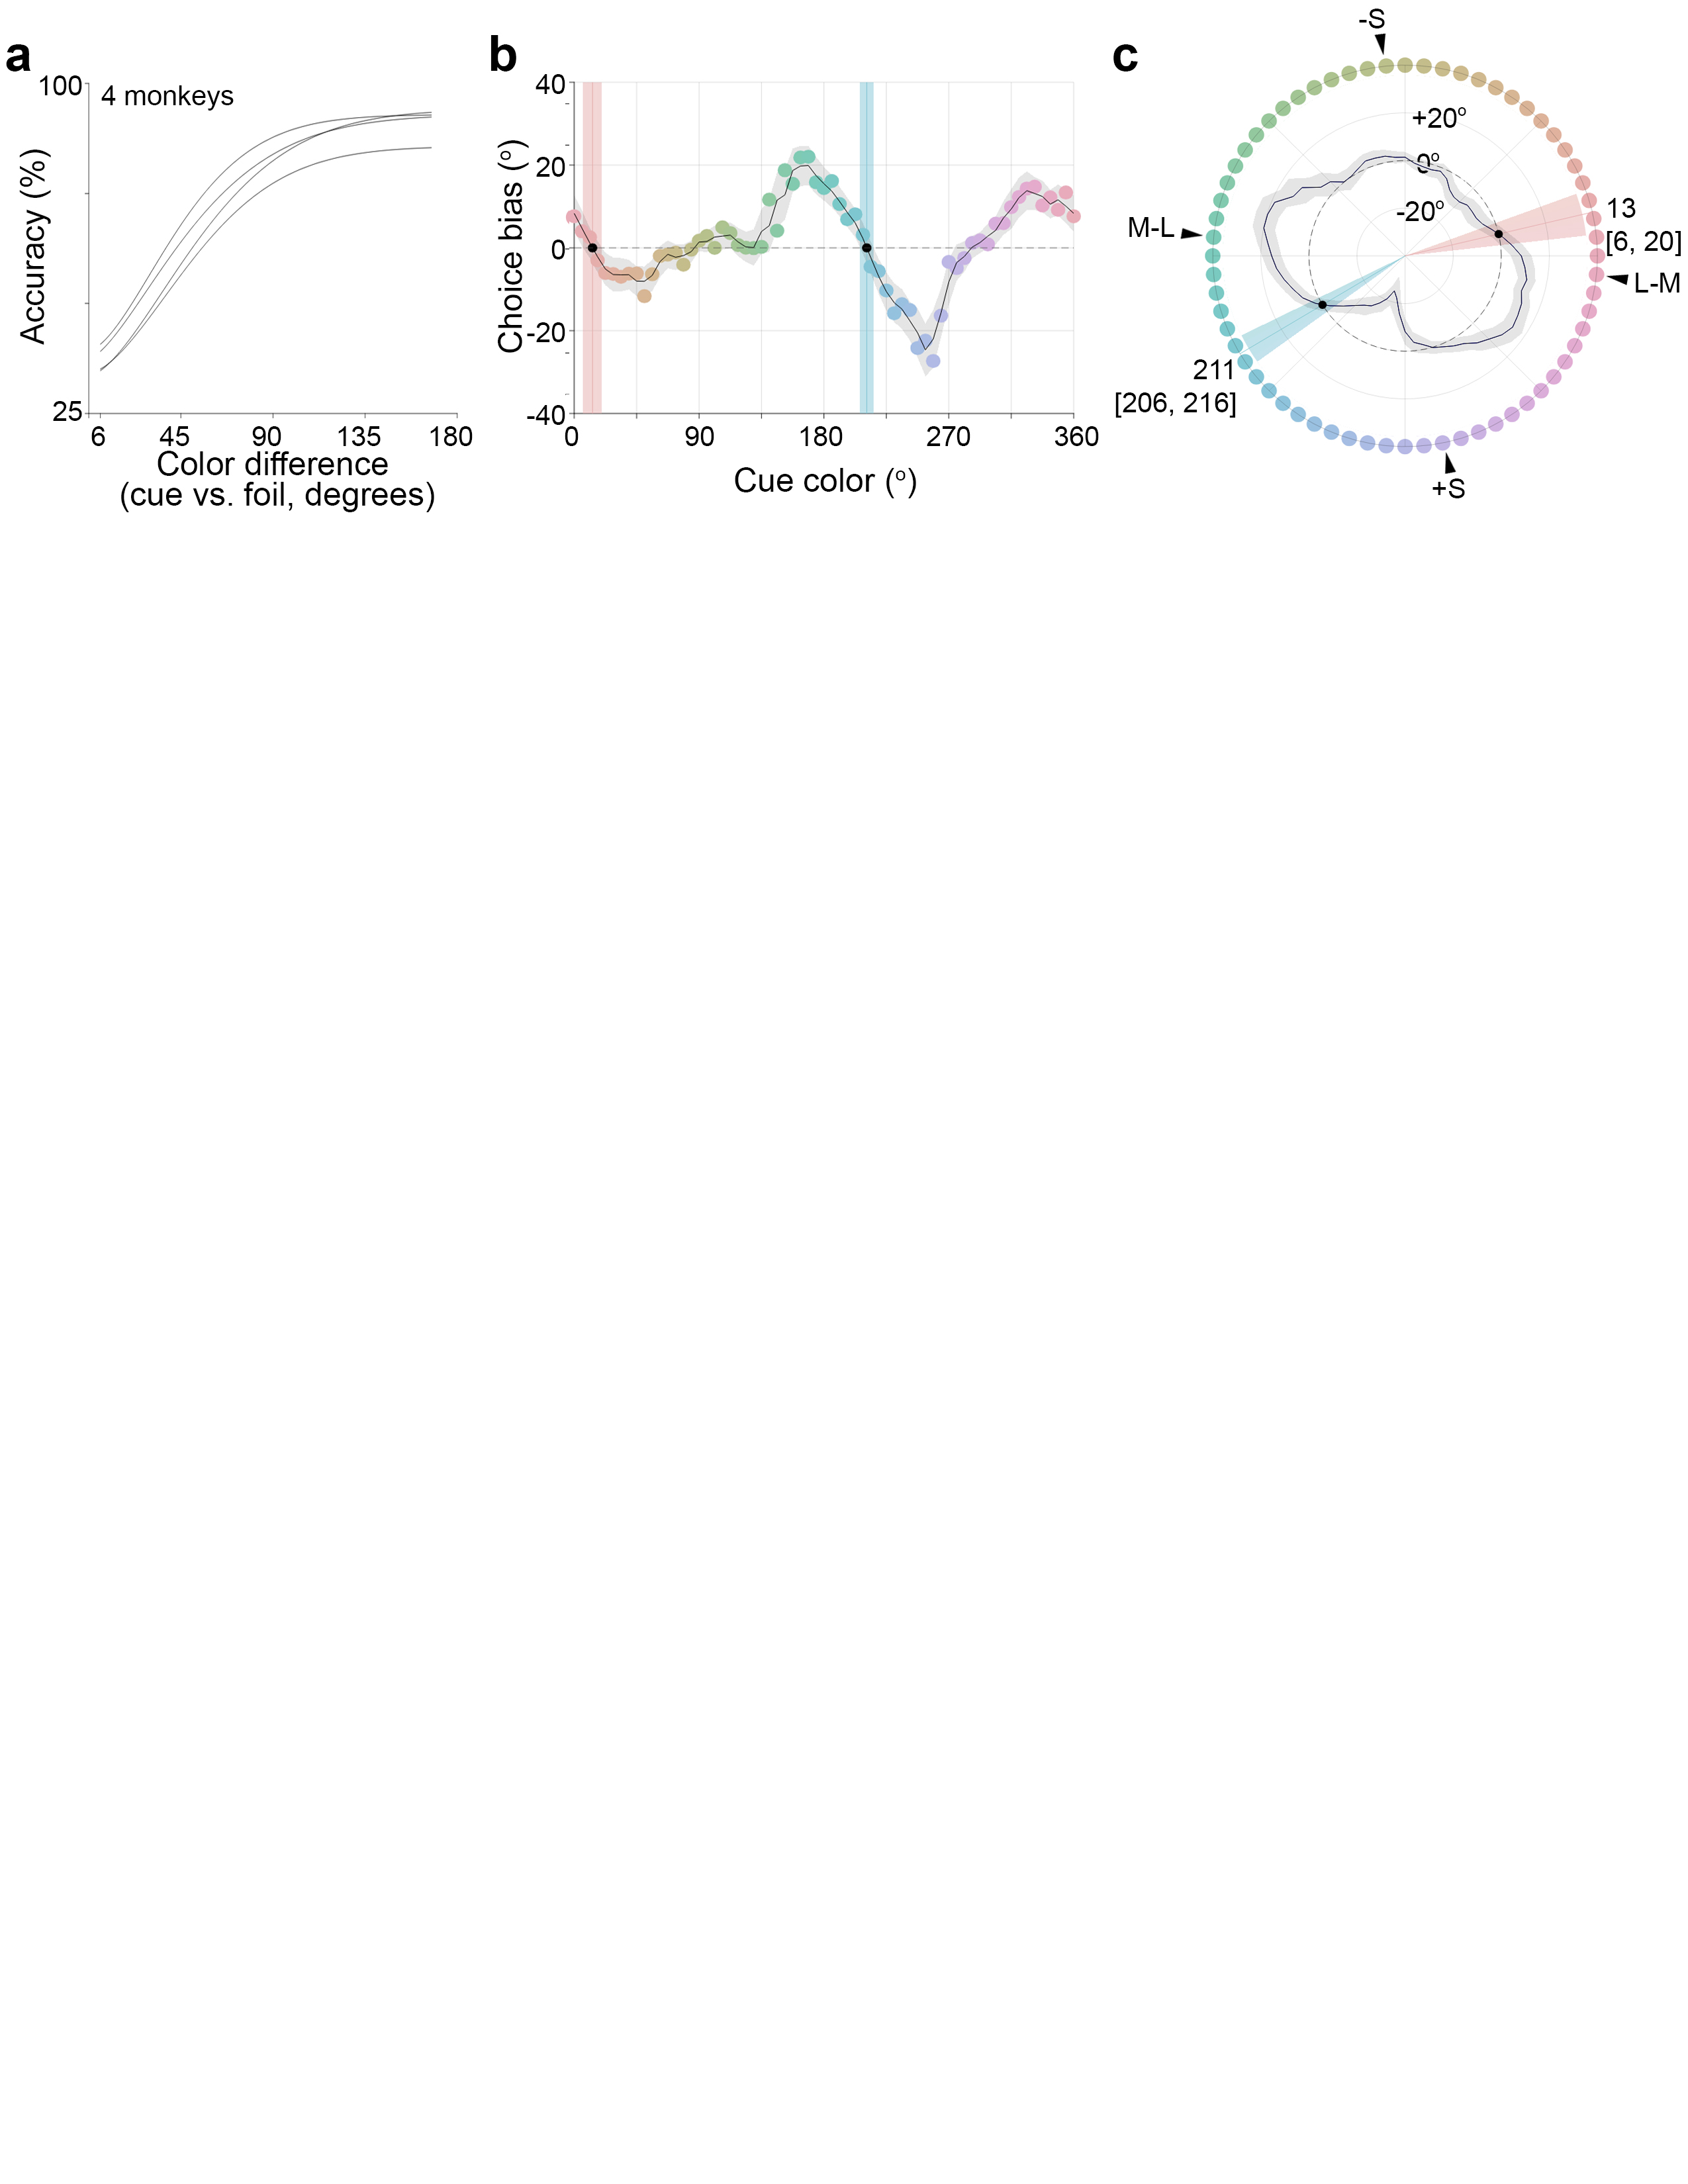
\includegraphics[width=\textwidth+4cm,trim={0 20cm 0 0},clip]{../Figures/flat/F2_CombinedMMResults_5.jpg}
    \caption{\textbf{Macaque monkeys appear to show two consensus color categories when the data are analyzed with a mixture model that computes the average distribution of the choices for each cue.}
	\textbf{a}, Psychometric functions for the four animals showing the accuracy of the matches as a function of the difference in hue angle between the cue and the foil that is closest in color to the cue. 
	The easiest trials were defined as those where the foil color nearest to the cue color were almost on the opposite side of the color circle. See SI Figure 2 for 95\% CI. 
	\textbf{b}, Mixture model results averaged across the four animals. The data were subsampled so that the same number of completed trials for each animal (24526) were included in the analysis. Error shading shows 95 \%CI. 
	The data recover two significant negative-slope zero-crossings (black dots), corresponding to two color categories. 
	\textbf{c}, Polar plot of the results in (b) with the zero crossings of the negative slope (following the trace counterclockwise) again indicated by black dots. The angle of the two inferred color categories [95 \% C.I.] are 13 [6, 20] (a peach color) and 211 [206, 216] (a teal color). }
    \label{fig:AvResults}
    \end{fullwidth}
\end{figure}

The four animals performed well on the task, achieving a lapse rate of 7\%, 7.1\%, 5.8\%, 14.3\% (Figure 2a; the plots of individual animals showing 95\% CI are provided in SI Figure 1). The results averaged across the four animals, analyzed using the mixture model as used previously to analyze data collected in humans \citep{bae_why_2015,zhang_discrete_2008} (see Methods), provided clear evidence of choice biases (Figure 2, SI Figure 3). But the consensus color categories inferred using this analysis do not support any of the predictions: the animals appeared to show two consensus color categories, not four as in humans. To the extent that the macaque is an accurate model of a non-linguistic human, these results show that the four color categories manifest in humans are not innate. The centers of the two apparent consensus color categories recovered in the monkeys were at angle 13 (a peach color) and 211 (a teal color). All four animals showed evidence of these two color categories (SI Figure 4).

\paragraph{Two possible explanations for choice biases in macaque monkeys}

\begin{figure}
    \begin{fullwidth}
    \centering
    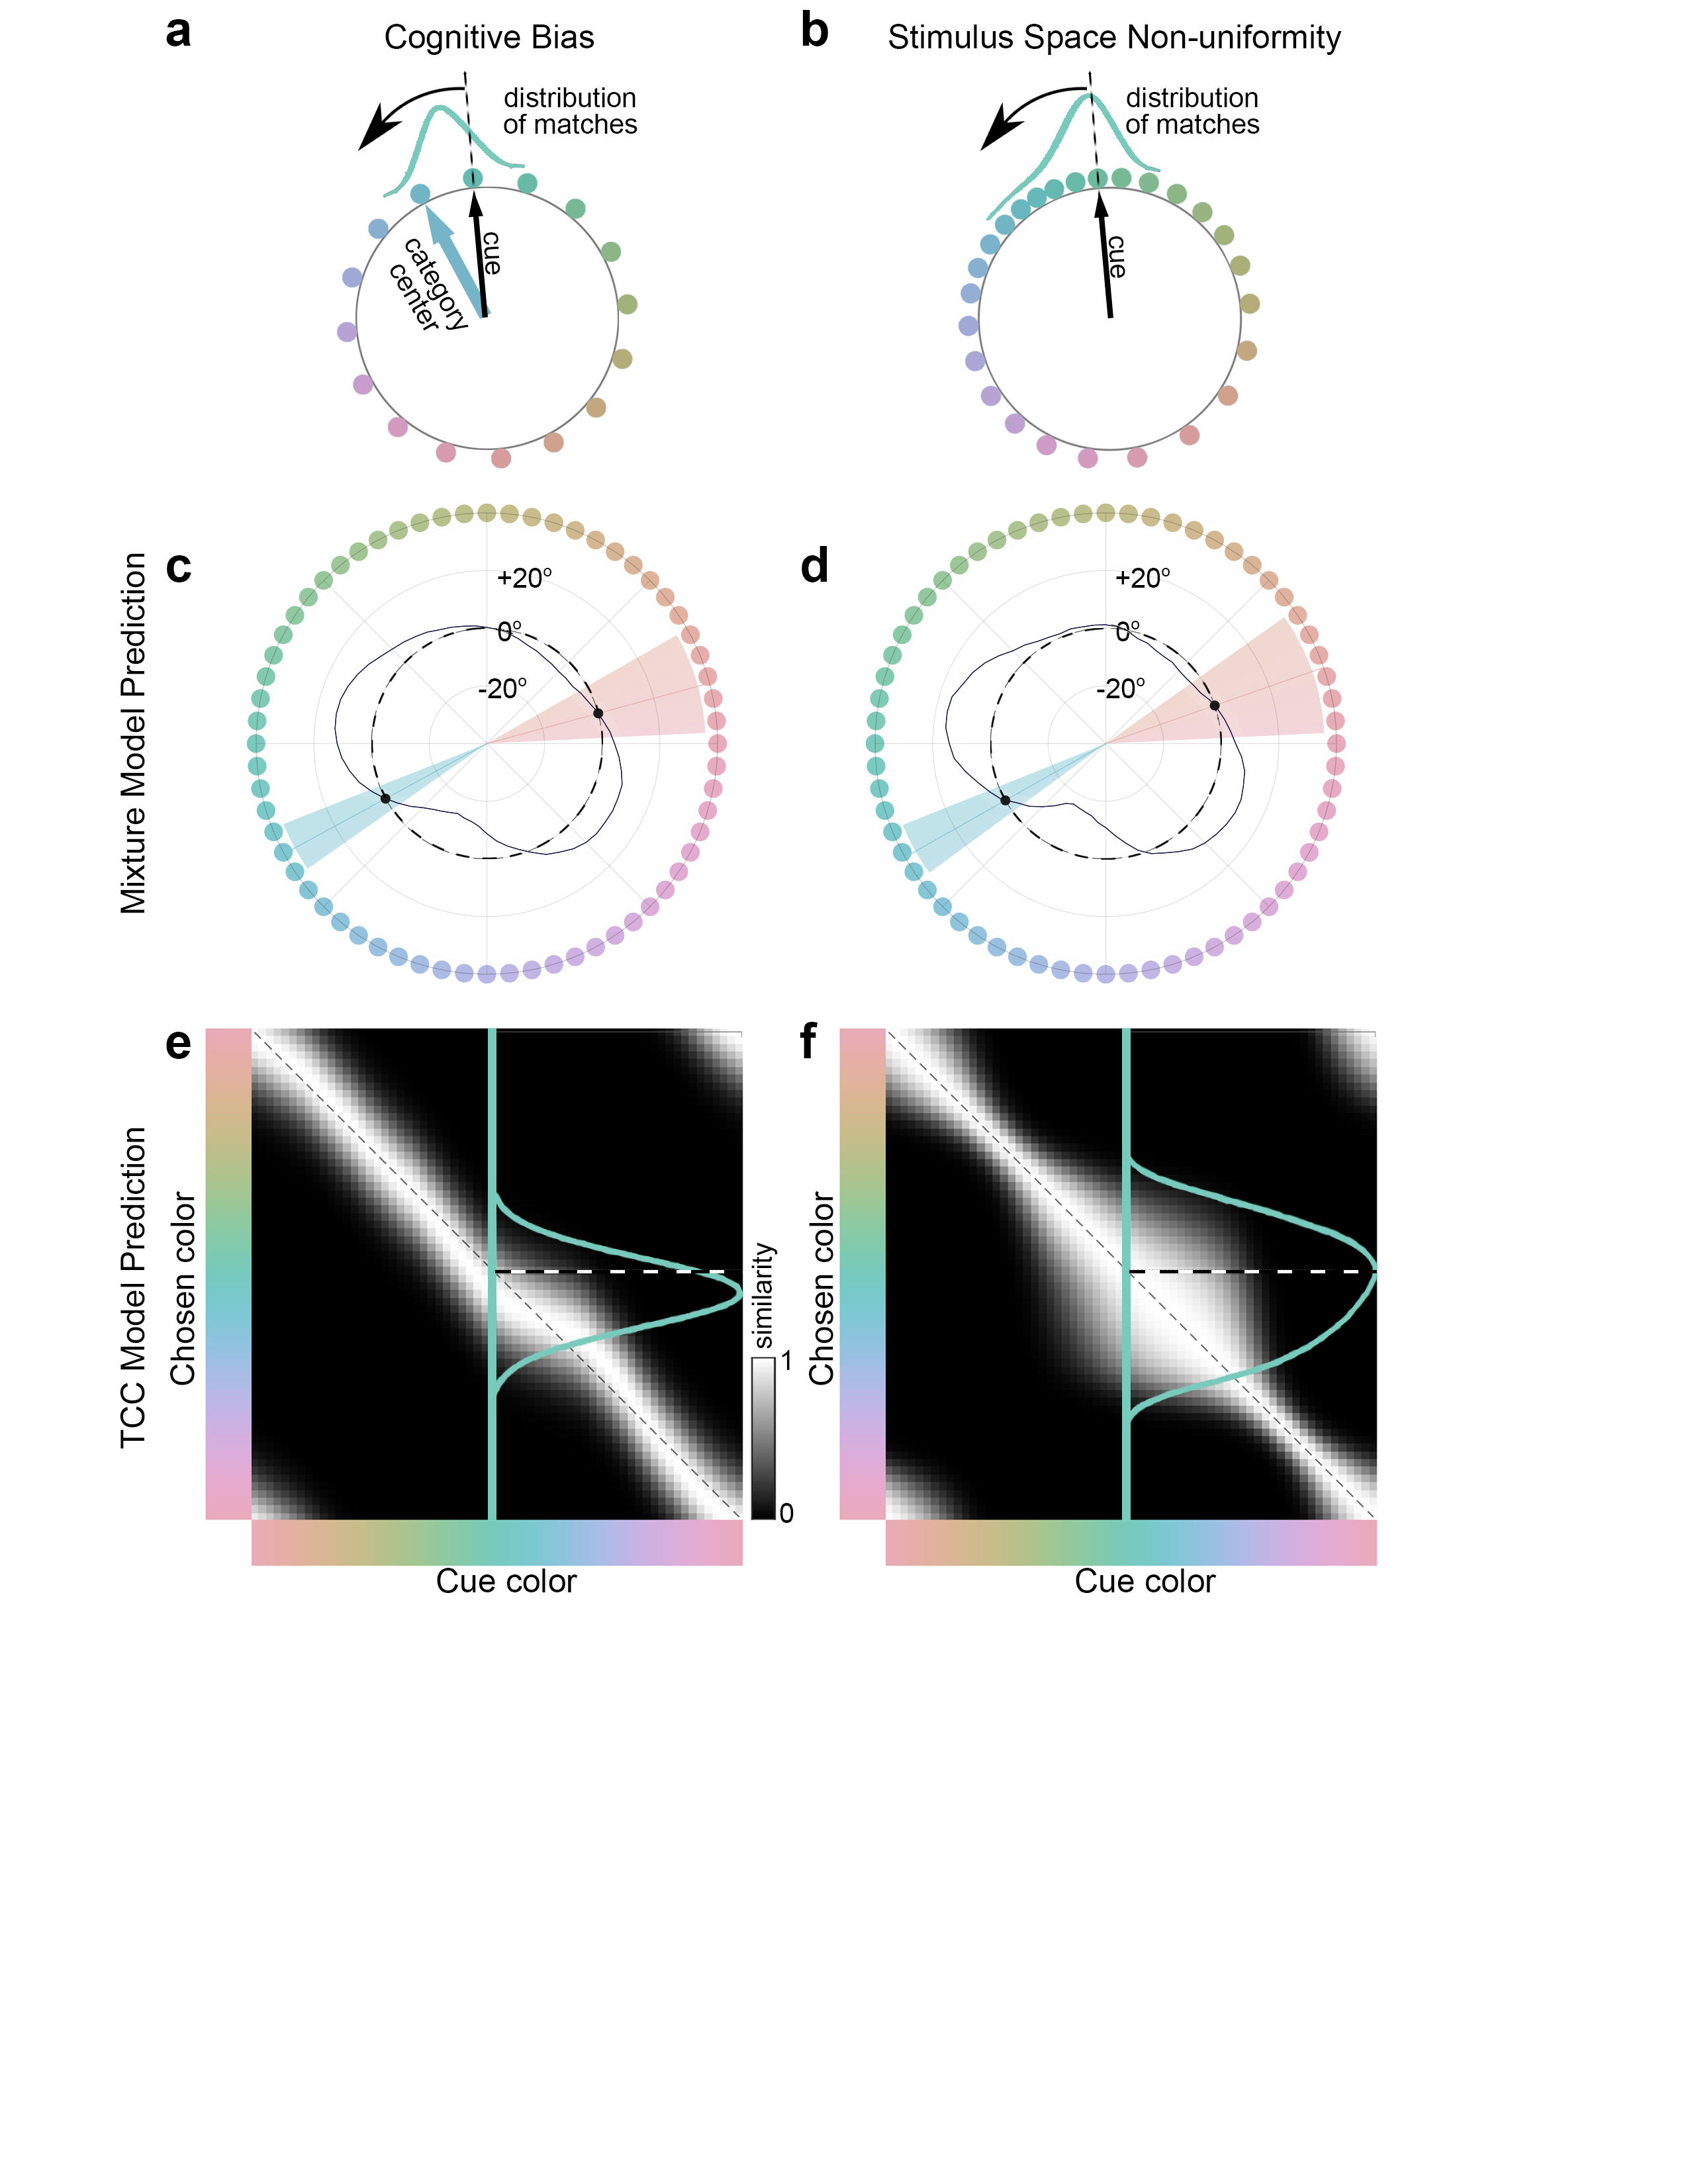
\includegraphics[width=\textwidth,trim={0 7cm 0 0},clip]{../Figures/flat/F3_TCCModel_6.jpg}
    \caption{\textbf{Computational simulations showing that color choice biases recovered by mixture model \citep{zhang_discrete_2008, bae_why_2015} could be explained by a non-uniformity in the stimulus space, without invoking cognitive mechanisms.} \textbf{a}, Color matches made by an agent with a cognitive color category, using a paradigm with stimuli that uniformly sample a truly uniform perceptual color space (gray circle). The distribution of matches has a peak biased towards the category center. \textbf{b}, Color matches made by an agent lacking a cognitive color category, with stimuli that non-uniformly sample an underlying uniform color space (gray circle). The distribution of matches is biased towards the densely sampled region of the space because there are more choice options. The average of the distribution of matches is similarly biased counterclockwise to the cue in both a and b, although the similarity functions differ in shape. \textbf{c}, Mixture-model analysis of a simulated data set with a cognitive bias; \href{https://github.com/NEI-LSR/MacaqueColorCategories/blob/main/Outputs/Paper/Figures/working/F3_TCCModel/Code/F3ace_TCCModel_OffsetGaussian.m}{Code for F3c} \textbf{d}, Mixture-model analysis of a simulated data set with a stimulus space non-uniformity. \href{https://github.com/NEI-LSR/MacaqueColorCategories/blob/main/Outputs/Paper/Figures/working/F3_TCCModel/Code/F3bdf_TCCModel_StimulusSpaceNonUnifomity.m}{Code for F3d}
    \textbf{e}, Similarity matrix for the simulated data analyzed in c; axes are CIELUV color space. Each column shows the similarity function for the corresponding cue on the x axis. The trace shows the similarity function for the cue in a. Note that the shape of the similarity function is symmetric like the distribution of matches. \href{https://github.com/NEI-LSR/MacaqueColorCategories/blob/main/Outputs/Paper/Figures/working/F3_TCCModel/Code/F3ace_TCCModel_OffsetGaussian.m}{Code for F3e} \textbf{f}, Similarity matrix for the simulated data analyzed in panel d; other details as in e. \href{https://github.com/NEI-LSR/MacaqueColorCategories/blob/main/Outputs/Paper/Figures/working/F3_TCCModel/Code/F3bdf_TCCModel_StimulusSpaceNonUnifomity.m}{Code for F3f}. The shape of the similarity function is different in e and f, yet both have the same mean bias relative to the cue. The similarity function in f and the distribution of matches in b are both asymmetric but differ in shape because the color spaces are different in b and f.}
    \label{fig:TCCDemo}
    \end{fullwidth}
\end{figure}

The colors we used were defined by the International Commission on Illumination (CIELUV) to be perceptually uniform. 
But it has long been recognized that there may be non-uniformities in all color spaces, including this one \citep{stockman_colorimetry_2010}; some authors have argued that perceptual uniformity may be task-dependent or simply unattainable \citep{judd_ideal_1969}. One might even suppose that if language influences color perception, as stipulated by the cultural-relativity hypothesis \citep{roberson_color_2005}, then all color spaces generated by human observers could be shaped by language. Could the macaque consensus color categories be attributed not to a true cognitive category (Figure 3a) but to unrecognized distortions in the presumed uniform space of colors (Figure 3b)? Both explanations could introduce biases in the distribution of matches (the mean for the distribution of matches will be biased away from the cue, curved arrows Figure 3a and 3b ).

The difference in the two explanations can be understood by considering the relationship between two neighboring colors in the color space. For the cognitive-bias account, there is an asymmetry between neighbors if there is a category center nearby. The color further from the category center will be more likely mistaken for the color closer to the category center than the other way around. Whereas for the non-uniform color space, there is no asymmetry in mismatches between neighboring colors. Both explanations lead to a distribution of matches that is shifted away from the cue. A cognitive bias would yield symmetric distributions of constant width for all cues around the color circle, but the distribution peaks would deviate from their respective cues depending on the proximity of the category center. A stimulus space non-uniformity, meanwhile, would yield an asymmetric distribution that varies in width depending on sampling density of the true underlying uniform color space, with regions that are relatively densely sampled having broader distributions. We refer to the distributions of matches for a given cue, plotted in CIELUV, as the similarity function for that cue, and the family of similarity functions for all cues as the similarity matrix (see hypothetical similarity matrices in Figure 3e and 3f; the turquoise trace shows one similarity function). 

To illustrate that the behavioral data could be explained by either a cognitive-bias account or a stimulus-space non-uniformity, we generated two sets of simulated data. One data set was generated with a simulation that used a uniform space and a bias arising from two cognitive categories, and the other data set was generated with a simulation that used non-uniform sampling of an underlying uniform color space and no cognitive categories. The data sets from both simulations gave rise to the same pattern of results when analyzed with a mixture model \citep{zhang_discrete_2008, bae_why_2015} (Figure 3c and 3d). These simulated data sets were chosen for illustration purposes because they correspond to the pattern of behavioral results (compare the simulated results in Figures 3c,d, with Figure 2c). 

To decide which of these explanations best accounts for the macaque behavioral data, we developed computational simulations and analyzed the data with an extension of the Target Confusability Competition (TCC) model \citep{schurgin_psychophysical_2020} (see Methods). 
The standard implementation of the TCC model assumes the same similarity function for each color. The version developed presently starts with a simpler version of the TCC model (replacing the two parameters for the similarity function with one, see Methods), and then allowing the shape and/or location of the similarity function relative to the cue to vary as a function of color (we refer to the modified TCC model as TCC-v, for "vary"). Let's consider three versions of the TCC-v model. First, the simplest (“null”) model has the same similarity function for each color, centered on the target color (this is conceptually equivalent to the original TCC model). Second, the "cognitive bias" version of the model specifies similarity functions for each color with peaks that can deviate from the target color but in which all similarity functions for the set of colors have the same symmetric (Gaussian) shape (Figure 3a). The result is a similarity matrix that has a band of constant width along the inverse diagonal but deviates to one side at color-category locations in the color space (Figure 3e). Third, the "stimulus-space non-uniformity" version of the model has a similarity function for each target color that fixes the peak to the target color but where the angular distances between the colors can differ for different colors. This results in a similarity matrix that is symmetric about the inverse diagonal, but which bulges out away from the diagonal at locations in the color space that are oversampled (Figure 3f). The stimulus-space non-uniformity model and the cognitive-bias model have the same number of parameters. 

To recap, the similarity matrix in 3e is constructed using the same data as the polar plot in 3c; and the similarity matrix in 3f is constructed using the same data as the polar plot in 3d. Panels c,d use the standard mixture-model approach which does not allow the shapes of the similarity functions to vary among the colors. Panels e,f, use the TCC-v approach, which permits the similarity functions to vary. The results of these computational simulations show that different underlying mechanisms could explain the appearance of choice biases in color-matching tasks when evaluated with the standard mixture model.

Next, we quantitatively compared the best fitting versions of each TCC-v model to the behavioral data. To facilitate this comparison, we plot the behavioral data with another version of the TCC-v model in which every cell in the similarity matrix is an independent model parameter ("free-similarity") (Figure 4a, 4b; the data for both panels are the same, centered on one or the other of the putative category centers recovered in the mixture model; free similarity matrices for the individual animals are shown in SI Figure 5). The free-similarity matrix makes no assumptions about the underlying mechanisms that determine the similarity between any pair of stimuli. Free similarity matrices provide similar information as choice probability matrices, but with more power. Each choice probability matrix (SI Figure 6) shows in each cell the proportion of times a given color was selected for each cue on all error trials. Now we can ask, are the data illustrated by the average free similarity matrix better explained by the stimulus space non-uniformity model or the cognitive bias model? In other words, do the panels in Figure 4a and 4b show mirror symmetry with bulges about the diagonal (like Figure 3f) or asymmetry about the diagonal without bulges (like Figure 3e)? 

\begin{figure}
    \begin{fullwidth}
    \centering
    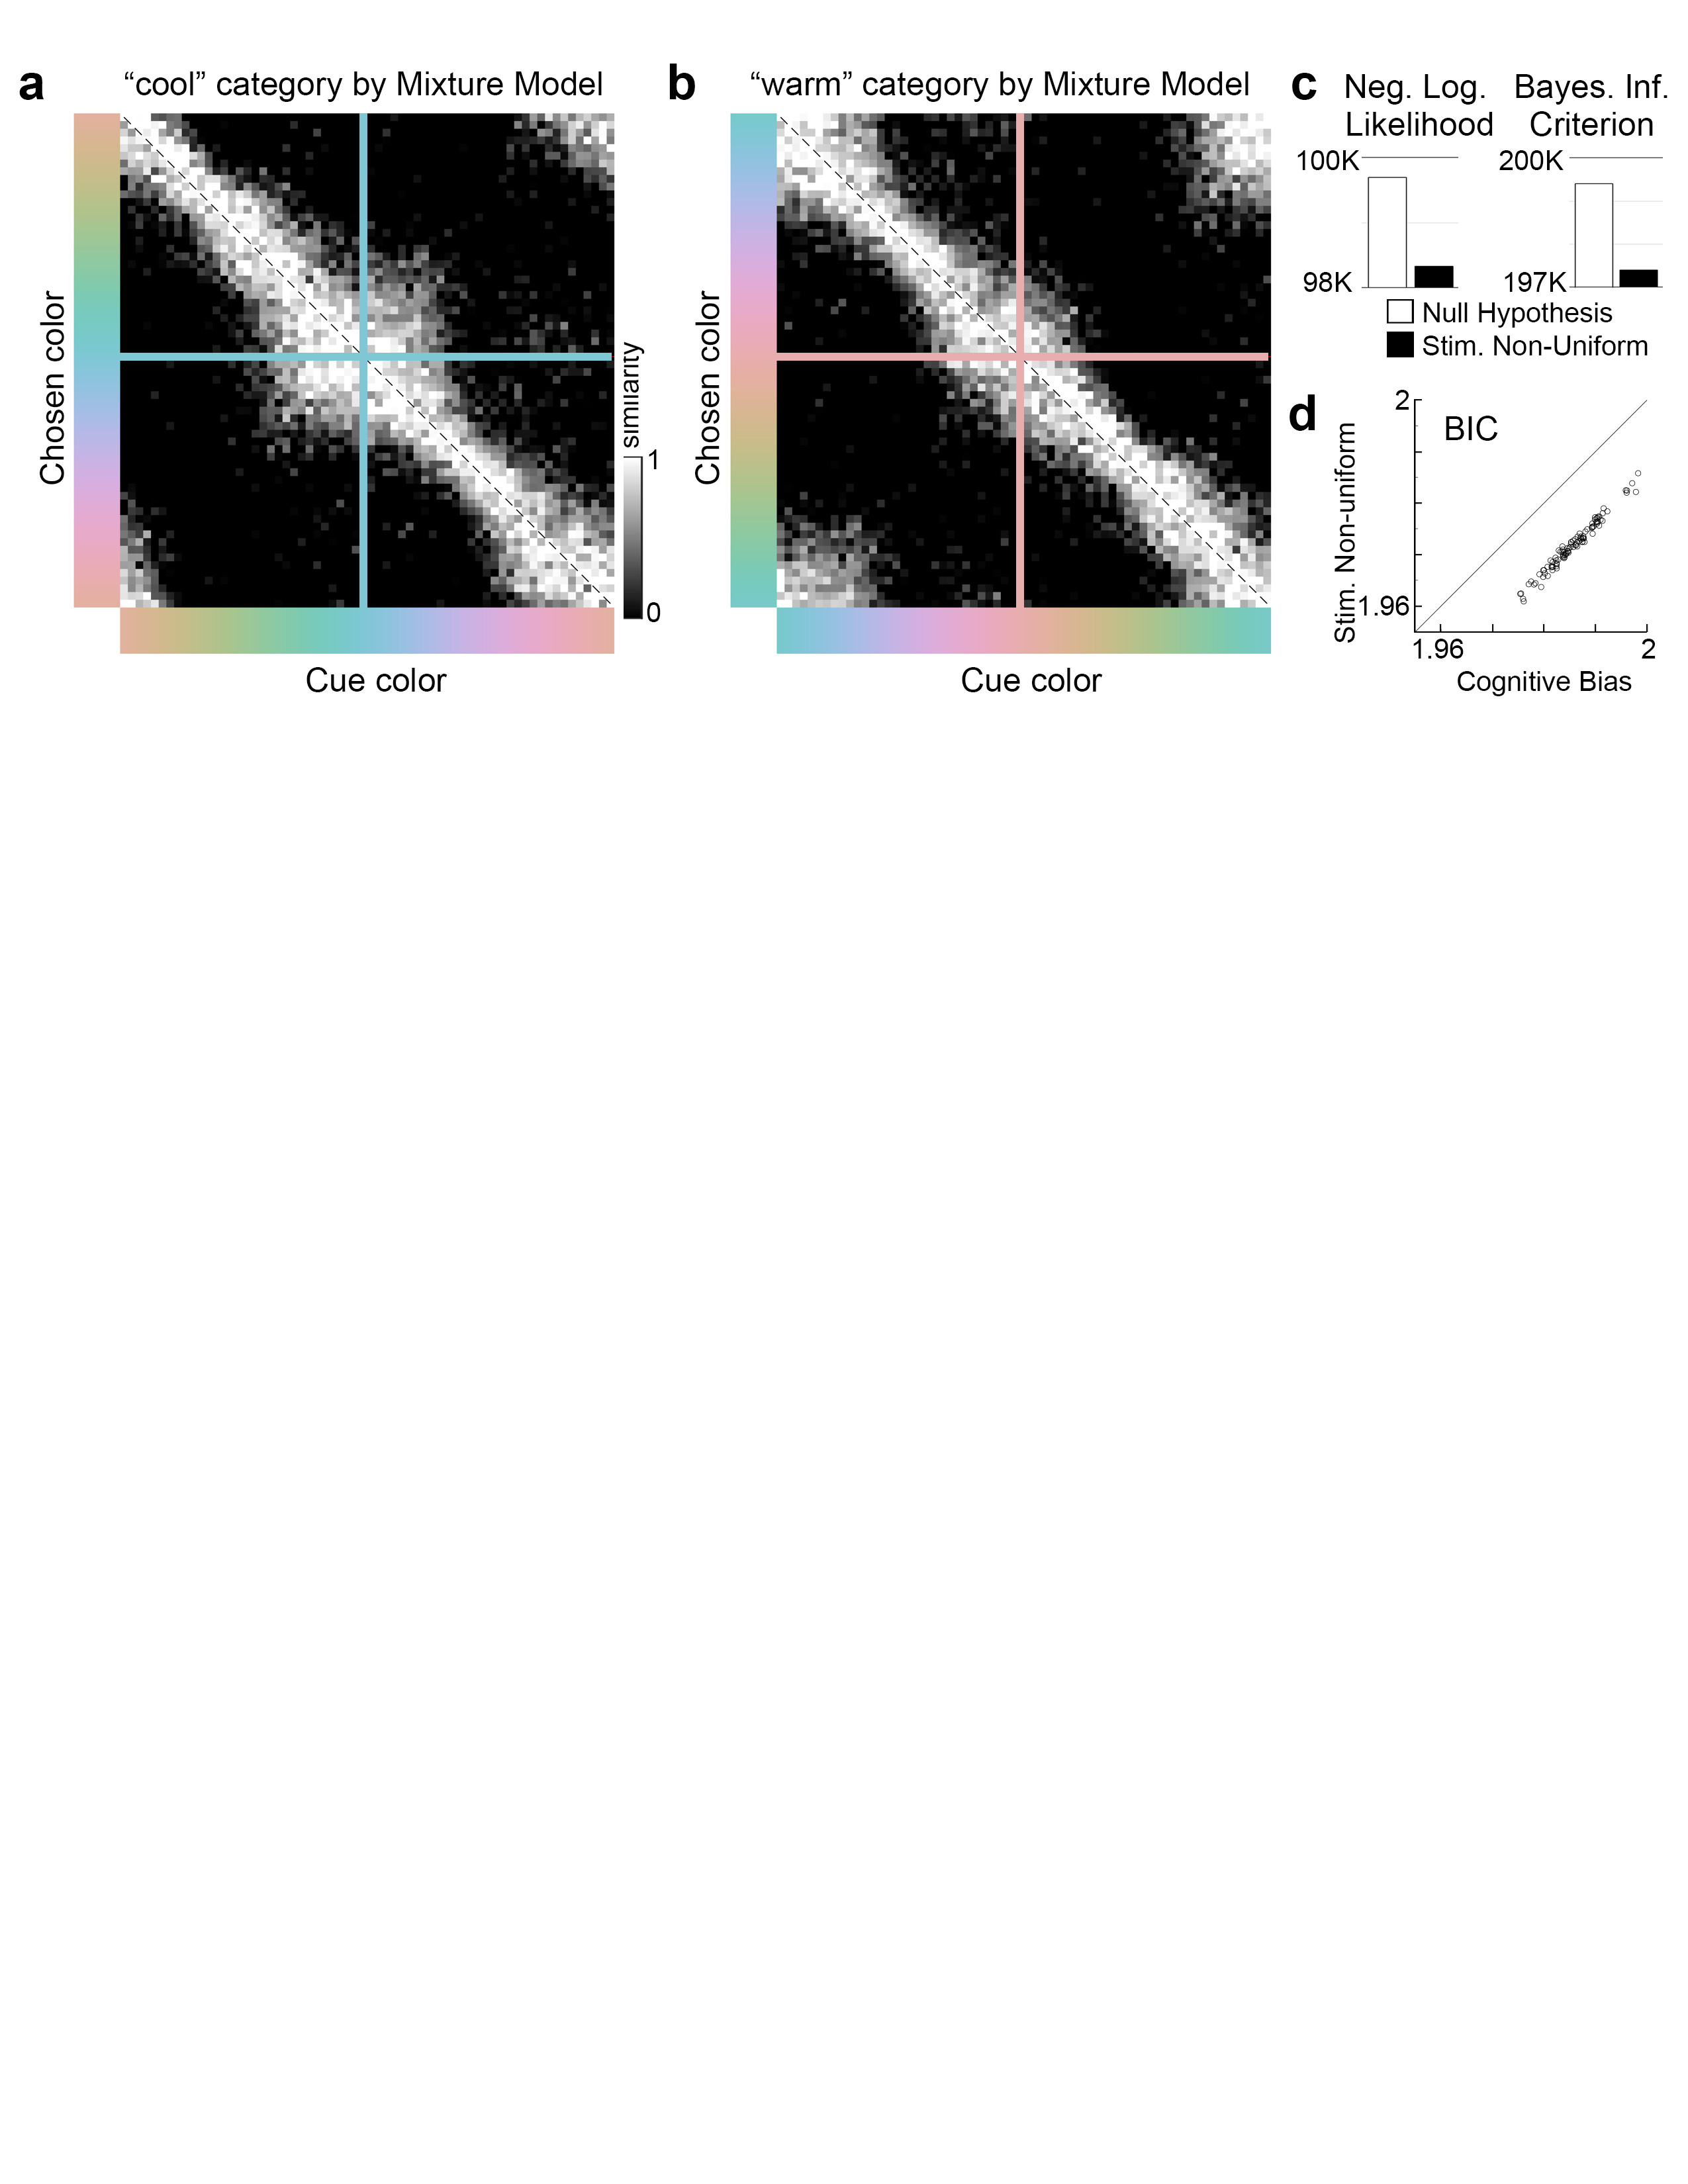
\includegraphics[width=\textwidth+4cm,trim={0 19cm 0 0},clip]{../Figures/flat/F4_TCCResults_3.jpg}
    \caption{\textbf{Similarity matrices for behavioral data averaged across four monkeys}
    \textbf{a}, Data centered on the teal-colored category recovered in the mixture model.  
	\textbf{b}, Data centered on the peach-colored category recovered in the mixture model. The pattern of results in a, b is better predicted by stimulus space non-uniformity (Figure 3f) than cognitive bias (Figure 3e). 
	\textbf{c}, Negative Log Likelihood (left) and Bayesian Inference Criterion (BIC, right) of the fit of the null model and the stimulus-space non-uniformity model. 
	\textbf{d}, BIC estimates of the fit provided by the stimulus-space non-uniformity model were always lower than BIC estimates of the fit for the cognitive bias model for 100 bootstrap repeats of the analysis. For each boostrap repeat, the number of trials for each animal were the same, set by the animal that completed the smallest total number of completed trials, and that number of trials was drawn with replacement from the total number of completed trials for each animal. The stimulus space non-uniformity model and the cognitive bias model have the same number of parameters. 
    } 
    \label{fig:TCCOutput}
    \end{fullwidth}
\end{figure}


By visual inspection, the data are better explained by the stimulus space non-uniformity model, a conclusion affirmed by statistical tests. First, the stimulus space non-uniformity model provides a better fit of the data than the null model (Figure 4c). Second, the data are better explained by the stimulus-space non-uniformity model than the cognitive bias model (Figure 4d). These results show that the apparent two consensus color categories recovered by the mixture model are explained by an unwitting non-uniformity in the underlying color space, and that the there is a non-linear mapping of a true perceptually uniform color space and the presumed uniform color space we used. These results therefore suggest that macaque monkeys do not have any innate consensus color categories. If the macaque is an accurate model of the human, then the results imply that humans do not have innate consensus color categories either. 

The data presented so far are for the four animals combined, which allowed us to assess the existence of consensus color categories. But we noted that the individual animals showed some idiosyncratic differences (SI Figure 4, SI Figure 5).
By mixture-model analysis, one animal showed not only the two consensus choice biases but also a third bias, for pea green (Figure 5a). The free similarity matrix for the data from this animal shows an asymmetry about the diagonal at this location in the color space (Figure 5b), showing that this animal has a cognitive bias for pea-green in addition to the consensus biases driven by stimulus-space non-uniformities. The result in this animal, and suggested by trends that the other animals also have idiosyncratic cognitive biases, show that macaque monkeys have the potential to form cognitive color biases, and that the TCC-v model can recover them. This is important not simply because it confirms that the ability to form cognitive categories does not require language \citep{panichello_error-correcting_2019}, but also because it shows that if macaques had consensus color categories, we would have been able to observe them.


\begin{figure}
    \begin{fullwidth}
    \centering
    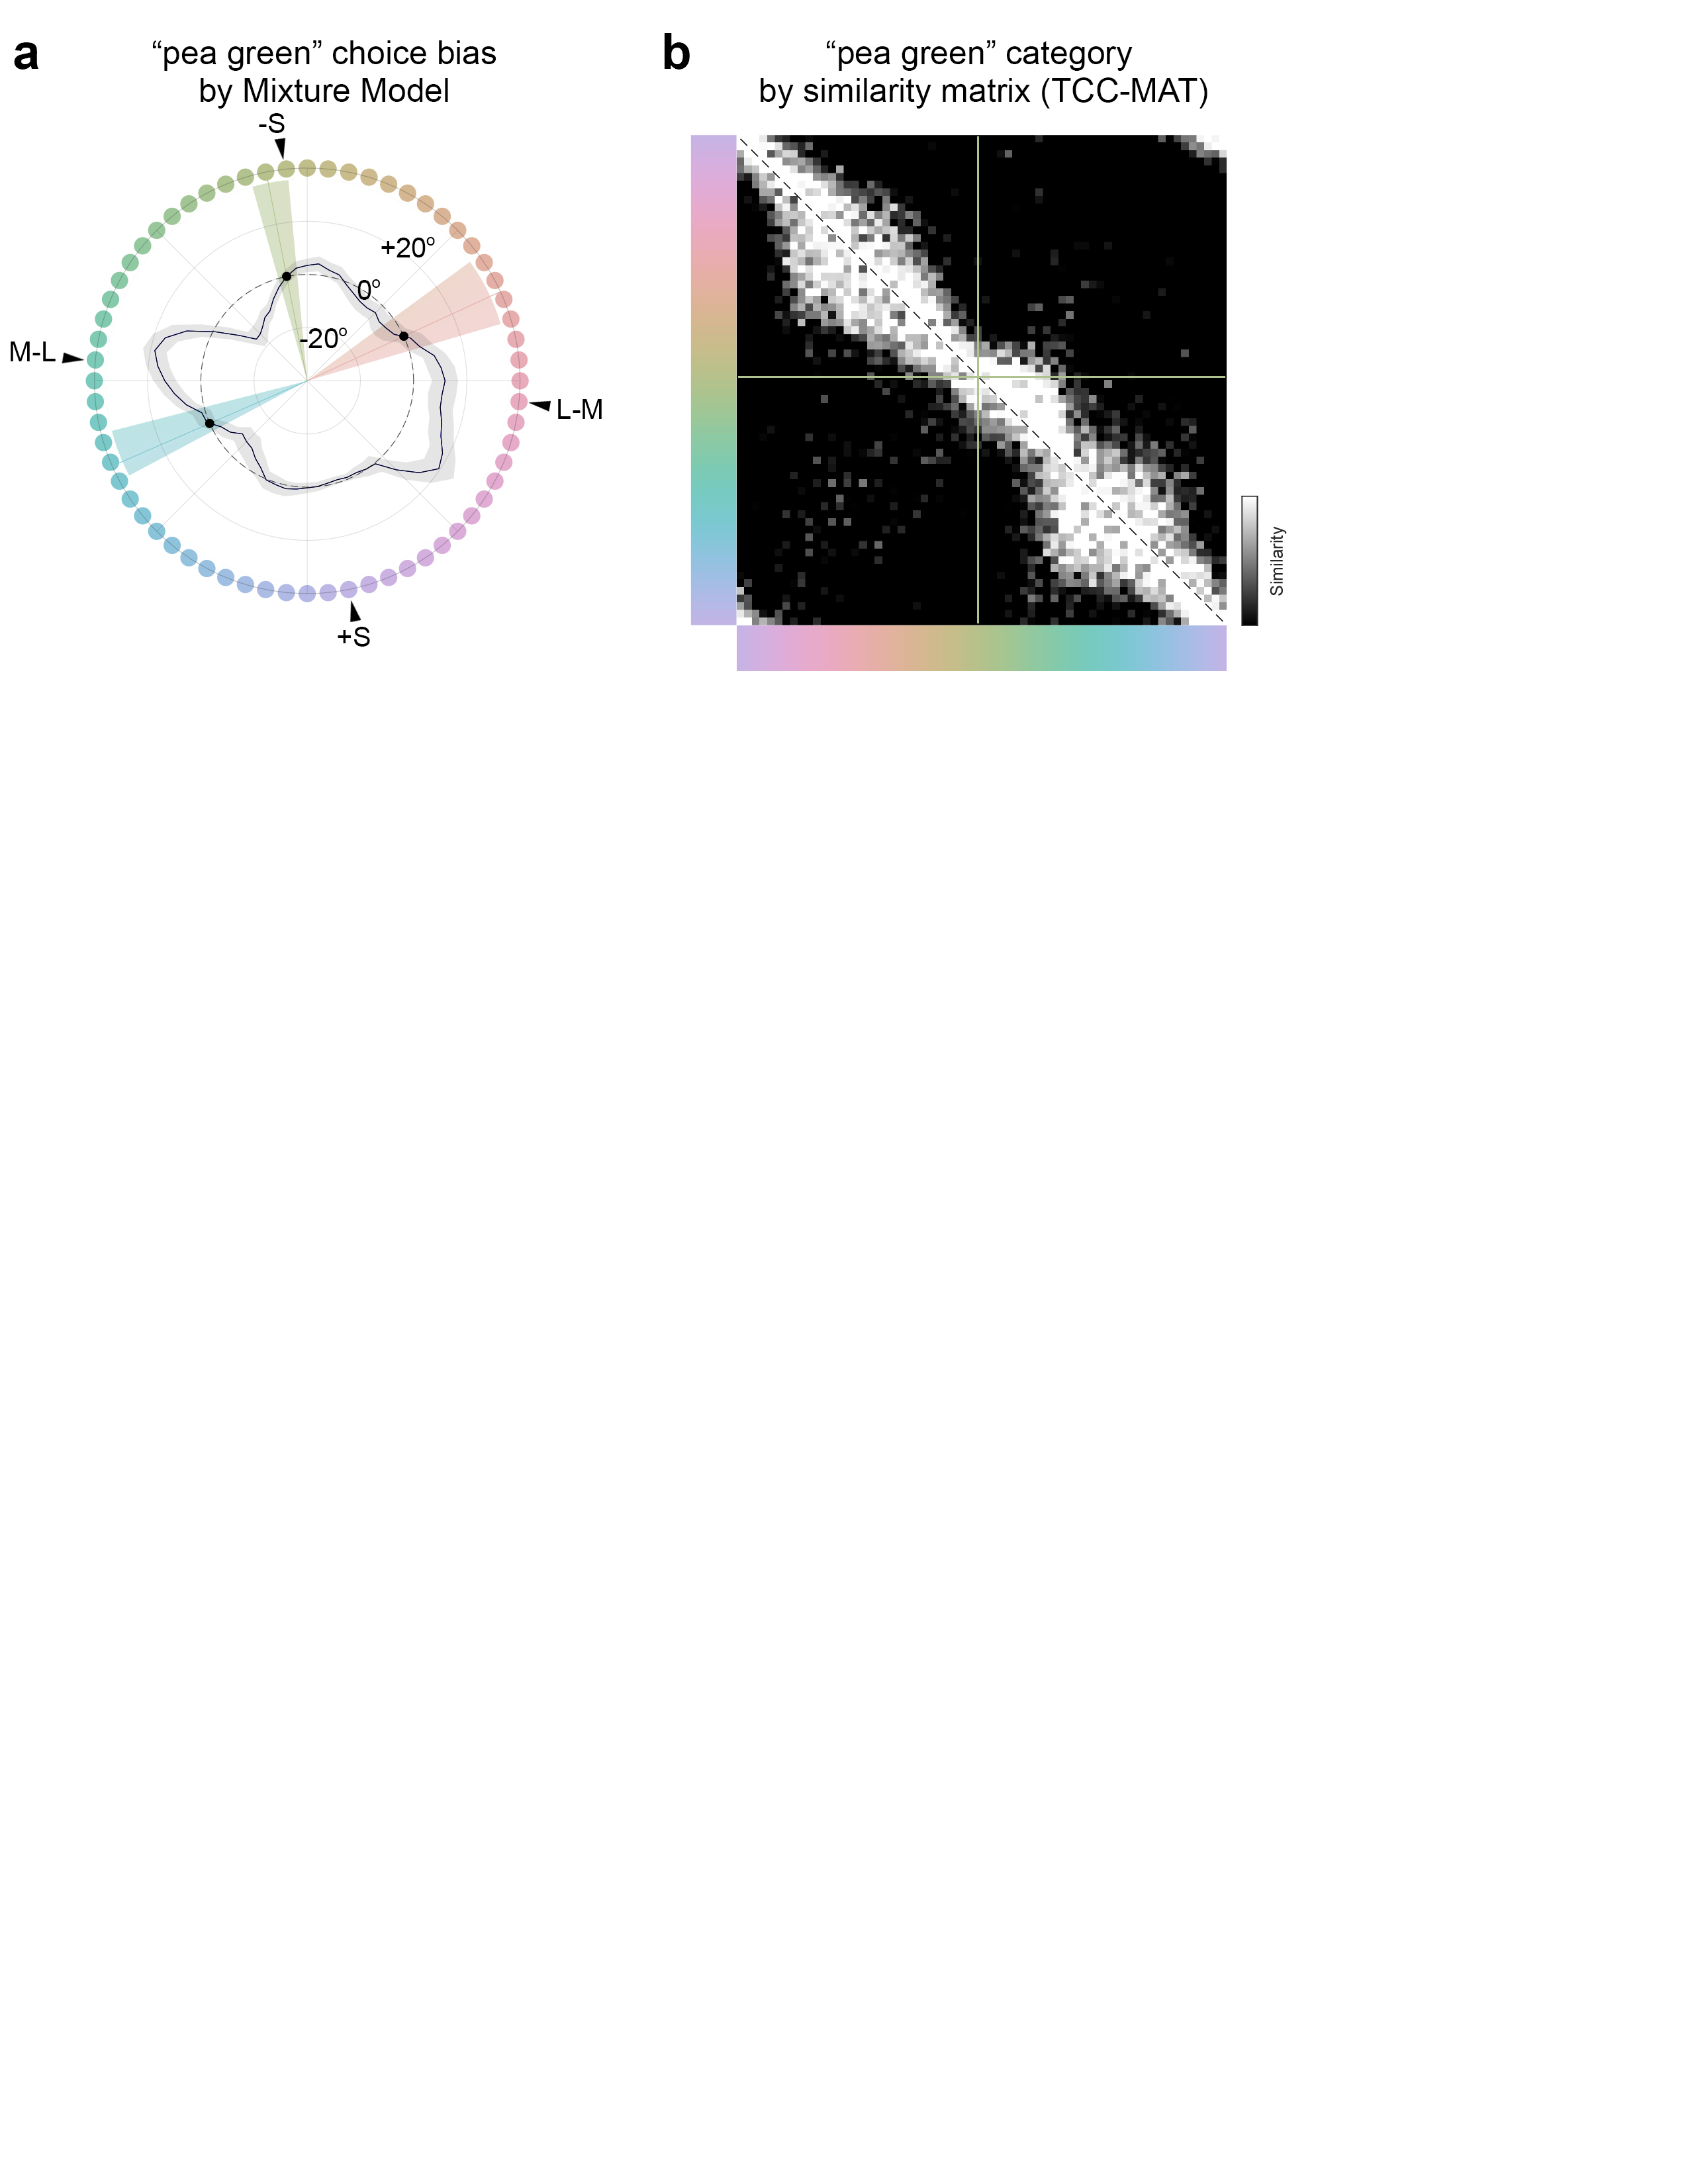
\includegraphics[width=\textwidth+4cm,trim={0 18cm 0 0},clip]{../Figures/flat/F5_CastorCogBias_6.jpg}
    \caption{\textbf {Color-matching data for one monkey showing evidence for a cognitive color category bias.} 
    \textbf{a}, Mixture-model analysis (same format as Figure 2c). 
	\textbf{b}, Free-similarity matrix (same format as Figure 4a,b) with an asymmetry in the green region indicated by the cross.}
    \label{fig:IndiDataCogBias}
    \end{fullwidth}
\end{figure}

\begin{figure}
    \begin{fullwidth}
    \centering
      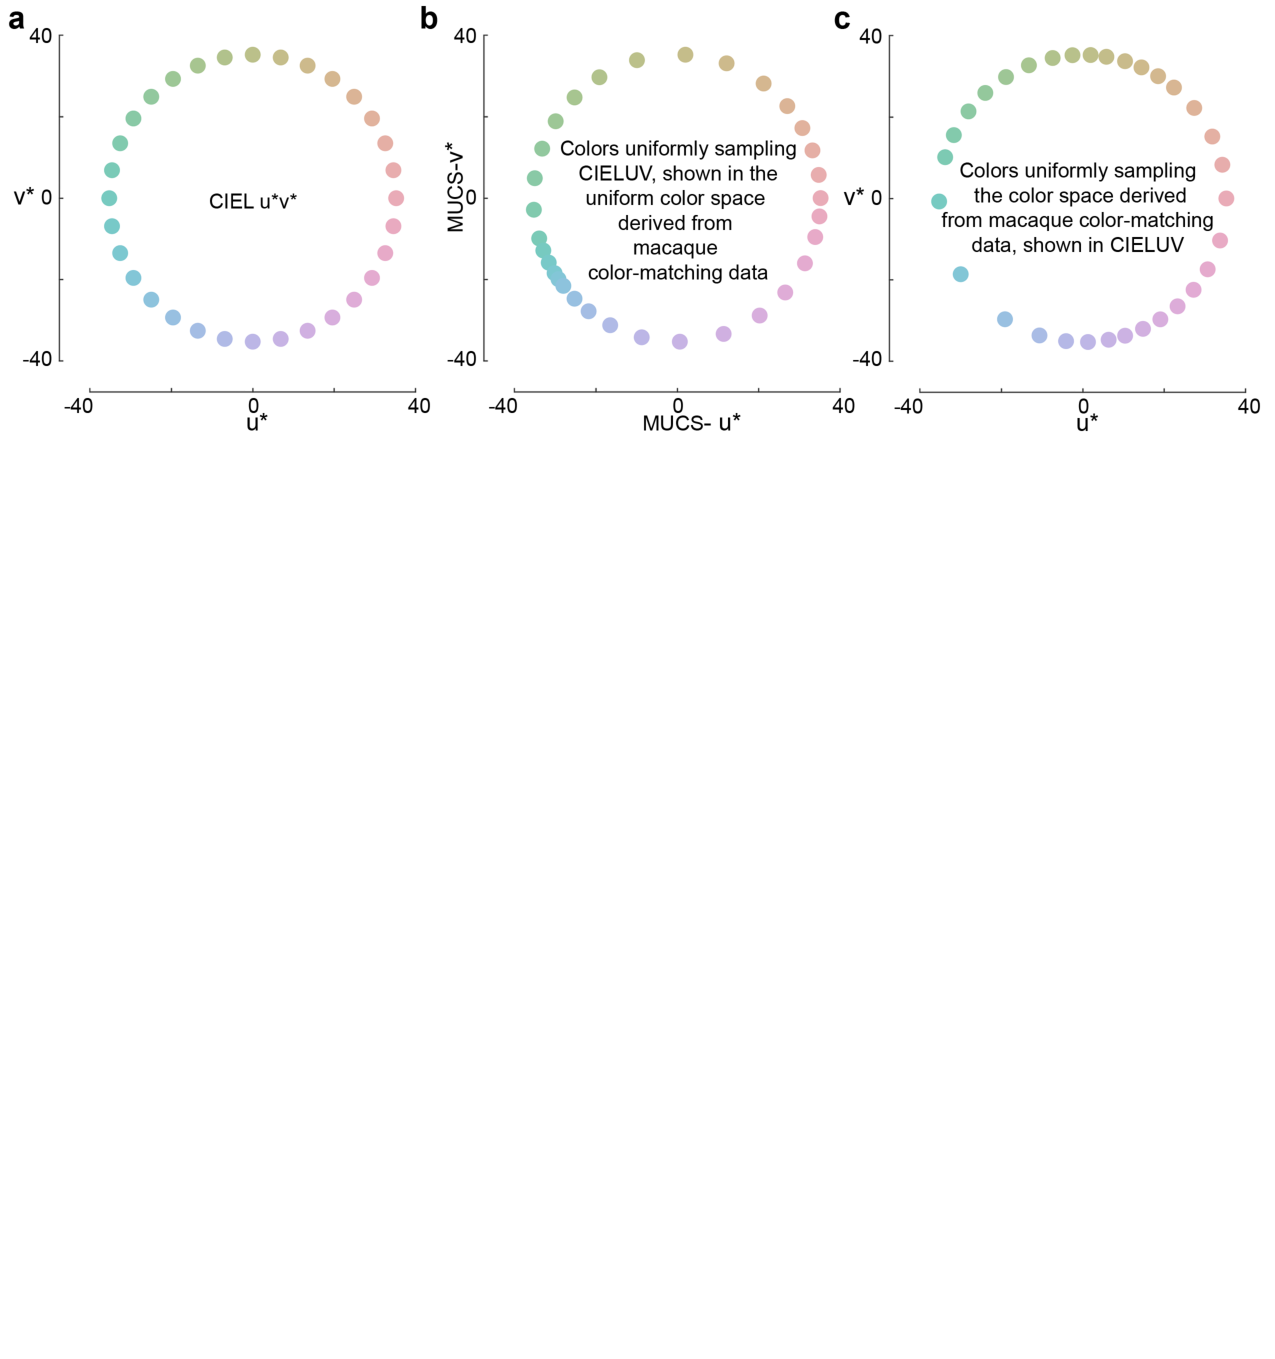
\includegraphics[width=\textwidth+4cm,trim={0 15cm 0 0},clip]{../Figures/flat/F6_ColSpace_2}
           \caption{\textbf{Perceptually uniform color space derived from the color-matching data in macaque monkeys.} 
			\textbf{a}, CIELUV color space with 64 color samples at even intervals in hue angle. 
			\textbf{b}, The same color samples plotted in the uniform color space derived from macaque monkeys; note that the axes are not CIELUV but MUCS (macaque uniform color space). 
			\textbf{c}, Colors sampled from evenly from the uniform color space derives from macaque monkeys, projected into CIELUV.}
		\label{fig:MACBEHcolorspace}
    \end{fullwidth}
\end{figure}


\paragraph{A perceptually uniform color space unconfounded by language}

The behavioral data in macaques provide a rare opportunity to reconstruct a perceptually uniform color space unconfounded by language. We computed, empirically, a transformed color space such that the macaques would, on average, show no choice bias. We refer to this space as the Macaque Uniform Color Space (MUCS). When colors evenly sampled from the CIELUV space (Figure 6a) are plotted within this macaque-derived uniform color space, colors are bunched around the teal part of the space, and to a lesser extent, around the peach-colored part of the space (Figure 6b). We can also take colors sampled at uniform intervals in MUCS and project them into CIELUV (Figure 6c). This arrangement shows relative bunching around lime colors and lavender colors, which correspond to the colors of the poles of the S-cone-opponent axes. These results provide clues to the origin of the stimulus space non-uniformity in CIELUV.

The mixture-model results in macaque monkeys are strikingly different from those in humans, insofar as the data in humans consistently recover evidence of four consensus categories, while the data in macaque monkeys show evidence of only two consensus categories. But the data in the two species are similar in one regard: they both show repeller points aligned with the poles of the S-cone axis (compare the zero crossings of the positive slopes in Figure 1e with those in Figure 2c; SI Figure 2) \citep{skelton_biological_2017,bae_why_2015,panichello_error-correcting_2019}. The repellor points indicate locations in the color space that are perceived but not readily allocated to a category. These results raise the possibility that the non-uniformity in CIELUV observed in supra-threshold color-matching tasks arise because the contribution of S-cone signals to color perception has not been accurately estimated for this task. Such an inaccuracy may reflect differences color spaces derived from threshold measurements versus appearance measurements, along with differences in the way S-cone signals, compared to L-M signals, are handled by the visual system \citep{RN655, conway_color_2014}. 

The present results imply that, contrary to longstanding arguments in empirical philosophy \citep{RN18743}, perception by itself is not sufficient to generate consensus color categories. Prior work has already shown that color perception is unnecessary for people to generate rich conceptual knowledge of color, including color categories: congenitally blind people have color concepts \citep{RN18700}. Taken together, we conclude that perception is neither necessary nor sufficient for the emergence of consensus color categories, and consensus color categories are therefore likely not innate. The present results are consistent with the idea that color ordering and the capacity to form color categories are innate. 

If color categories are not innate, where do they come from? Color categories appear to reflect the behavioral relevance of colors in the world \citep{RN18616,gibson_color_2017}; the relevance of things is partially culturally determined, introducing a role for language in shaping consensus color categories. Given that color categories can be learned, as clearly evident in at least one macaque in our study (Figure 5) and two macaques in another study \citep{panichello_error-correcting_2019}, the introduction of language provides a mechanism by which cultures can form consensus about color categories. For example, the parts of scenes labeled as objects are more likely to be warm colored while backgrounds are more likely to be cool colored \citep{rosenthal_color_2018}, and these statistics predict universal patterns in color naming \citep{gibson_color_2017}. We speculate that the choice biases in humans, which may include more than four consensus color categories (\citep{skelton_biological_2017}, and see note in legend for SI Figure 2), likely reflect cognitive biases, and that these achieve consensus through shared behavioral relevance that is communicated through language \citep{RN18511,RN18514,RN18602}. 
